
\documentclass[tikz,convert={convertexe={magick.exe}, density=800}]{standalone}
\usepackage{tikzsymbols}
\usepackage{MnSymbol,wasysym}

\begin{document}
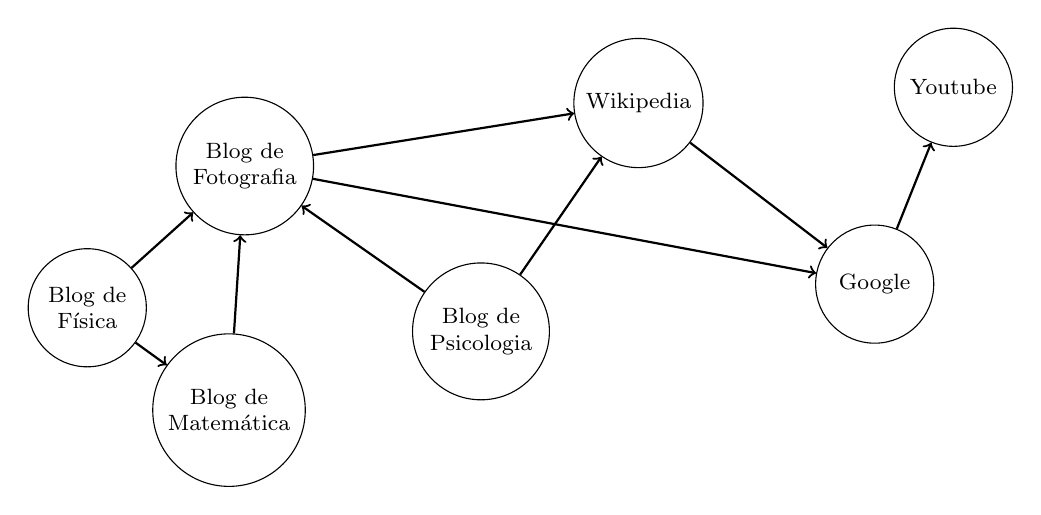
\begin{tikzpicture}[
page/.style={circle, draw, fill=white, minimum size=1.5cm, align=center, font={\footnotesize}},
link/.style={thick,->}
]

    
\node (W) at (0,0.8) [page] {Wikipedia};
\node (J1) at (-5,0) [page] {Blog de\\Fotografia};
\node (I) at (3,-1.5) [page] {Google};

\node (J2) at (-7, -1.8) [page] {Blog de\\Física};
\node (J3) at (-5.2, -3.1) [page] {Blog de\\Matemática};
\node (J4) at (-2, -2.1) [page] {Blog de\\Psicologia};

\node (D) at (4,1) [page] {Youtube};

\draw[link] (J2)--(J1);
\draw[link] (J3)--(J1);
\draw[link] (J4)--(J1);

\draw[link] (J1)--(W);
\draw[link] (J4)--(W);
\draw[link] (I)--(D);

\draw[link] (W)--(I);
\draw[link] (J1)--(I);
\draw[link] (J2)--(J3);


\end{tikzpicture}
\end{document}